\documentclass[aspectratio=1610]{beamer}
\usefonttheme{professionalfonts}
\usetheme{metropolis}
\setbeamertemplate{bibliography item}{\insertbiblabel}
\usepackage{polyglossia}
\setmainlanguage{english}
\usepackage{amsmath}
\usepackage{amssymb}
\usepackage{mathtools}
\usepackage{graphicx}
\usepackage[version=4]{mhchem}
\usepackage[
  math-style=ISO,
  bold-style=ISO,
  sans-style=italic,
  nabla=upright,
]{unicode-math}
\setmathfont{Latin Modern Math}
\usepackage{blindtext}
\usepackage{fontspec}
\title{}
\subtitle{}
\date{\today}
\author{Steven Becker}
\usepackage{siunitx}
\AtBeginDocument{
\sisetup{
math-rm=\mathrm,
math-micro=μ,
}
}
\usepackage{framed}
\usepackage{biblatex}
\addbibresource{lit.bib}
\usepackage{booktabs}

\begin{document}

%Chapters: 5.3.2.3, 7.3
%https://www.ncbi.nlm.nih.gov/pmc/articles/PMC3937800/
\frame{\maketitle}


\begin{frame}{Overview}
\begin{itemize}
  \setlength\itemsep{1.2em}
  \item{Virus detection in generell}
  \item{Photonic crystal}
  \item{Biosensing with 2D-PhCs}
\end{itemize}

\end{frame}

\begin{frame}{Virus detection in generell}
  \begin{itemize}
    \setlength\itemsep{1.2em}
    \item{\emph{Electron microscopy} - observe viruses in a sample   }
    \item{\emph{Gene sequencing} - out of a sample with millions of bases, you can detect the pathogen's bases   }
    \item{\emph{ Antibody detection} - immune system produce antibodies to fight the virus }
    \end{itemize}
\end{frame}

\begin{frame}{Photonic crystal}
  \begin{columns}

    \begin{column}{0.49\textwidth}
    \begin{itemize}
      \setlength\itemsep{1.2em}
      \item{periodic dielectric microstructure \, ( 1D, 2D and 3D)}
      \item{propagation of the electromagnetic wave depends on the wavelength}
      \item{characterized by their band structure }
    \end{itemize}
    \end{column}

    \begin{column}{0.49\textwidth}
    \begin{figure}
      \centering
      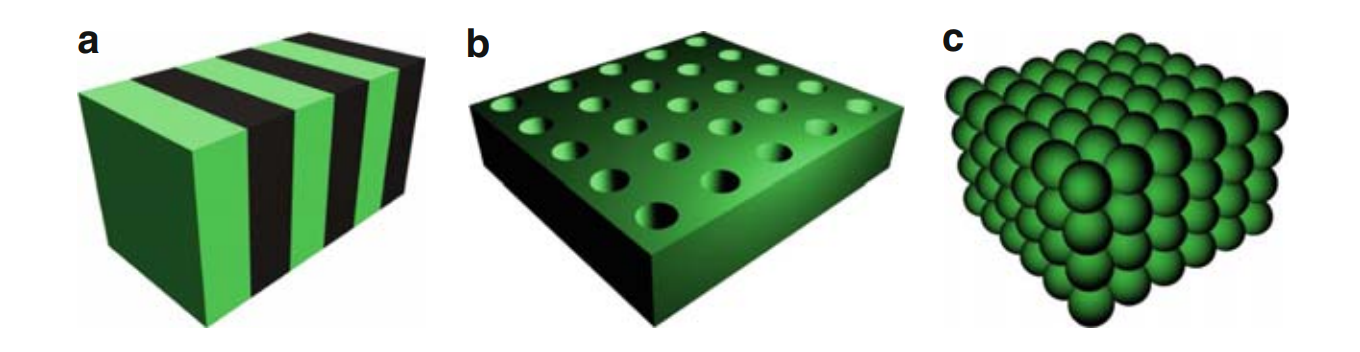
\includegraphics[width=1\textwidth]{./bilder/photonic_crystal_model.png}
      \caption{Example of 1D (a), 2D (b) and 3D (c) photonic chrystals. \cite{intro_pho}.}
      \label{fig: photonic_crystal}
    \end{figure}
  \end{column}

  \end{columns}

\end{frame}


\begin{frame}{Biosensing with 2D-PhCs}

  \begin{columns}

    \begin{column}{0.49\textwidth}
    \begin{itemize}
      \setlength\itemsep{1.2em}
      \item{\emph{structure + point + waveguide} - only one wavelength is absorbed (c. fig. \ref{fig: 2d_photonic_crystal} )}
      \item{ surface modification gives the option to detect a specific biological particle}
      \item { a redshift is observable}
    \end{itemize}
    \end{column}

    \begin{column}{0.49\textwidth}
    \begin{figure}
      \centering
      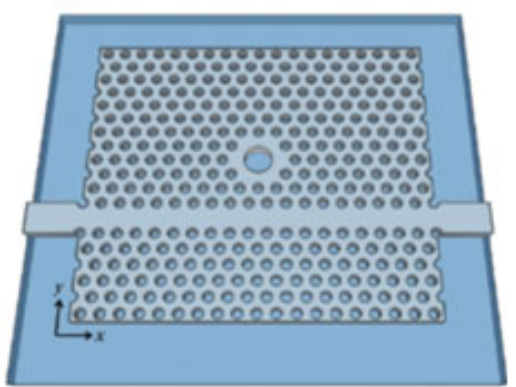
\includegraphics[width=0.8\textwidth]{./bilder/2dphc_waveguide_point_defect.png}
      \caption{2D photonic crystal with a punctually defect and a waveguide. \cite{nano}.}
      \label{fig: 2d_photonic_crystal}
    \end{figure}
  \end{column}

  \end{columns}

\end{frame}

\begin{frame}{Biosensing with 2D-PhCs}
  \begin{figure}
    \centering
    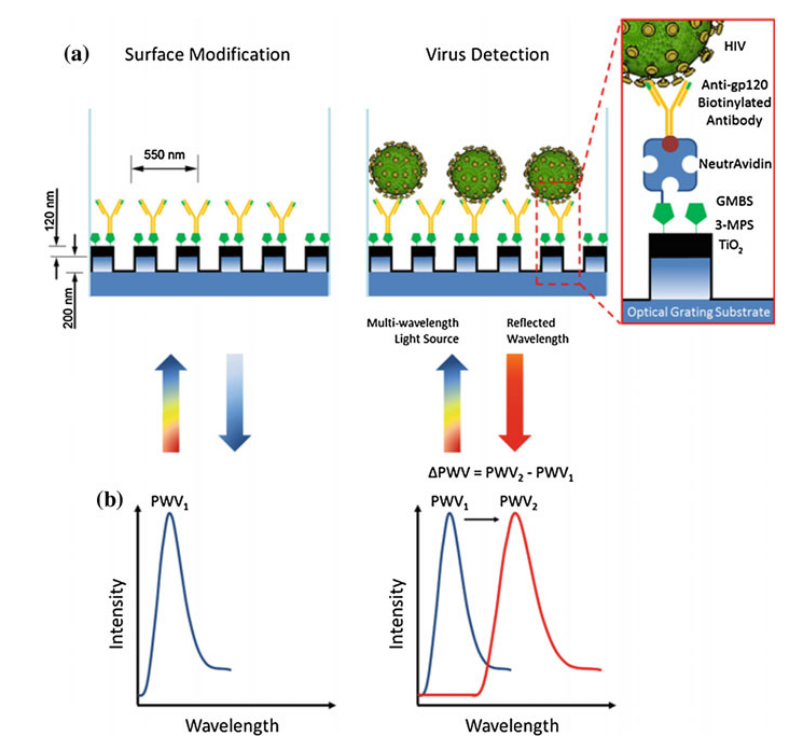
\includegraphics[width=0.5\textwidth]{./bilder/reflektion.png}
    \caption{Surface modification of a PhC allow a virurs detection. \cite{nano}.}
    \label{fig: virus detection}
  \end{figure}

\end{frame}

\begin{frame}
  \nocite{*}
  \printbibliography
\end{frame}
\end{document}
